\documentclass[aspectratio=169,12pt]{beamer}

\usepackage[utf8]{inputenc} % codificacao de caracteres
\usepackage[T1]{fontenc}    % codificacao de fontes
\usepackage[brazil]{babel}  % idioma
\usepackage{graphics}
\usepackage{helvet}

\usepackage{moresize}

\usepackage{tikz}
    \usetikzlibrary{positioning}

\let\tempone\itemize
\let\temptwo\enditemize

% Hide beamer navigation simbols
\beamertemplatenavigationsymbolsempty

% Use full screen
\hypersetup{pdfpagemode=FullScreen}

% Titulo
\title[\sc{Machine Learning}]{Machine Learning}
\subtitle{A fast and gentle introduction.}
\author[Prof. Jeffman]{Prof. Me. Rafael Guterres Jeffman}
\institute[FSPOA]{Faculdade Senac Porto Alegre} % opcional

\titlegraphic{
\includegraphics[width=.25\paperwidth]{images/fecomercio_senac.png}}
%\date{\today}
\date{}

% Center frame titles
\setbeamertemplate{frametitle}[default][center]

\setbeamertemplate{background canvas}[vertical shading][top=blue,bottom=black,middle=black!85!blue,midpoint=0.7]
\setbeamercolor{title}{fg=white}
\setbeamercolor{normal text}{fg=white}
\setbeamercolor{frametitle}{fg=white}
\setbeamercolor{structure}{fg=white}

\setbeamertemplate{items}[circle]

% Presentation content begins.
\begin{document}

\begin{frame}
    \titlepage
\end{frame}

{
 \usebackgroundtemplate{
  \centering
  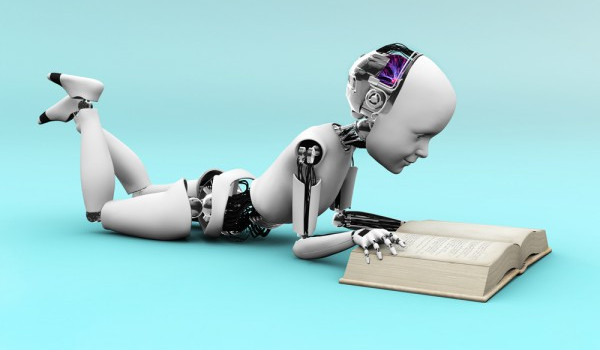
\includegraphics[width=\paperwidth]{images/droid-learning.jpg}
 }
\begin{frame}
    \begin{tikzpicture}[overlay,remember picture]
        \node[xshift=13cm, yshift=-4.75cm]
        {\tiny \color{black} Sarah Holmlund / Shutterstock};
    \end{tikzpicture}
\end{frame}
}


\begin{frame}
    \frametitle{Sistemas Inteligentes}
    \begin{itemize}
        \setlength\itemsep{1em}
        \item Apresentam comportamento inteligente.
        \item Apresentam respostas a problemas para
        os quais não foram programados.
        \item Sistemas capazes de dar uma resposta
        mesmo na ausência de informações.
    \end{itemize}
\end{frame}

{%
 \usebackgroundtemplate{
  \centering
  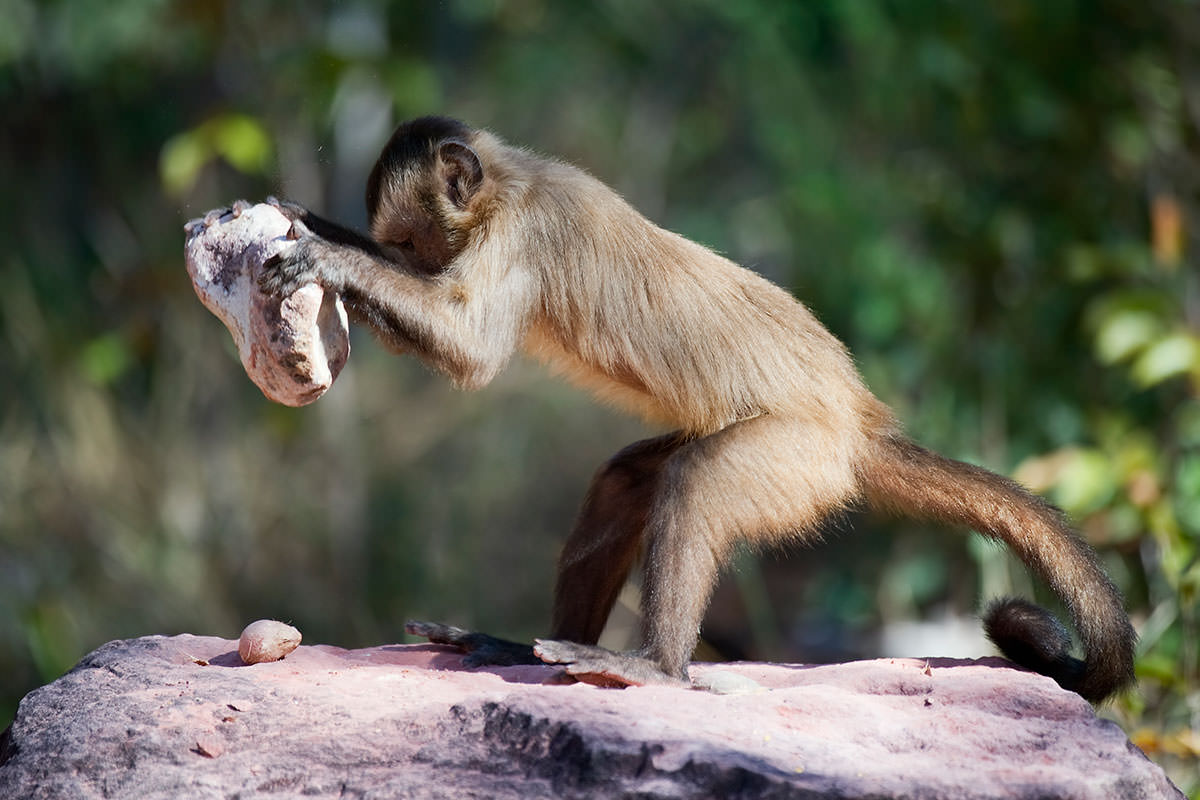
\includegraphics[width=\paperwidth]{images/monkey.jpg}
 }
 \begin{frame}[t]
  \begin{center}
    \color{white}{\textbf{\Huge O que é inteligência?}}
  \end{center}
    \begin{tikzpicture}[remember picture,overlay]
        \node [xshift=-1.2cm,yshift=0.5cm]
            [text width=3cm] at (current page.south east)
            {\tiny{Ben Cranke/Getty Images}};
    \end{tikzpicture}
 \end{frame}
}

{%
 \usebackgroundtemplate{
  \centering
  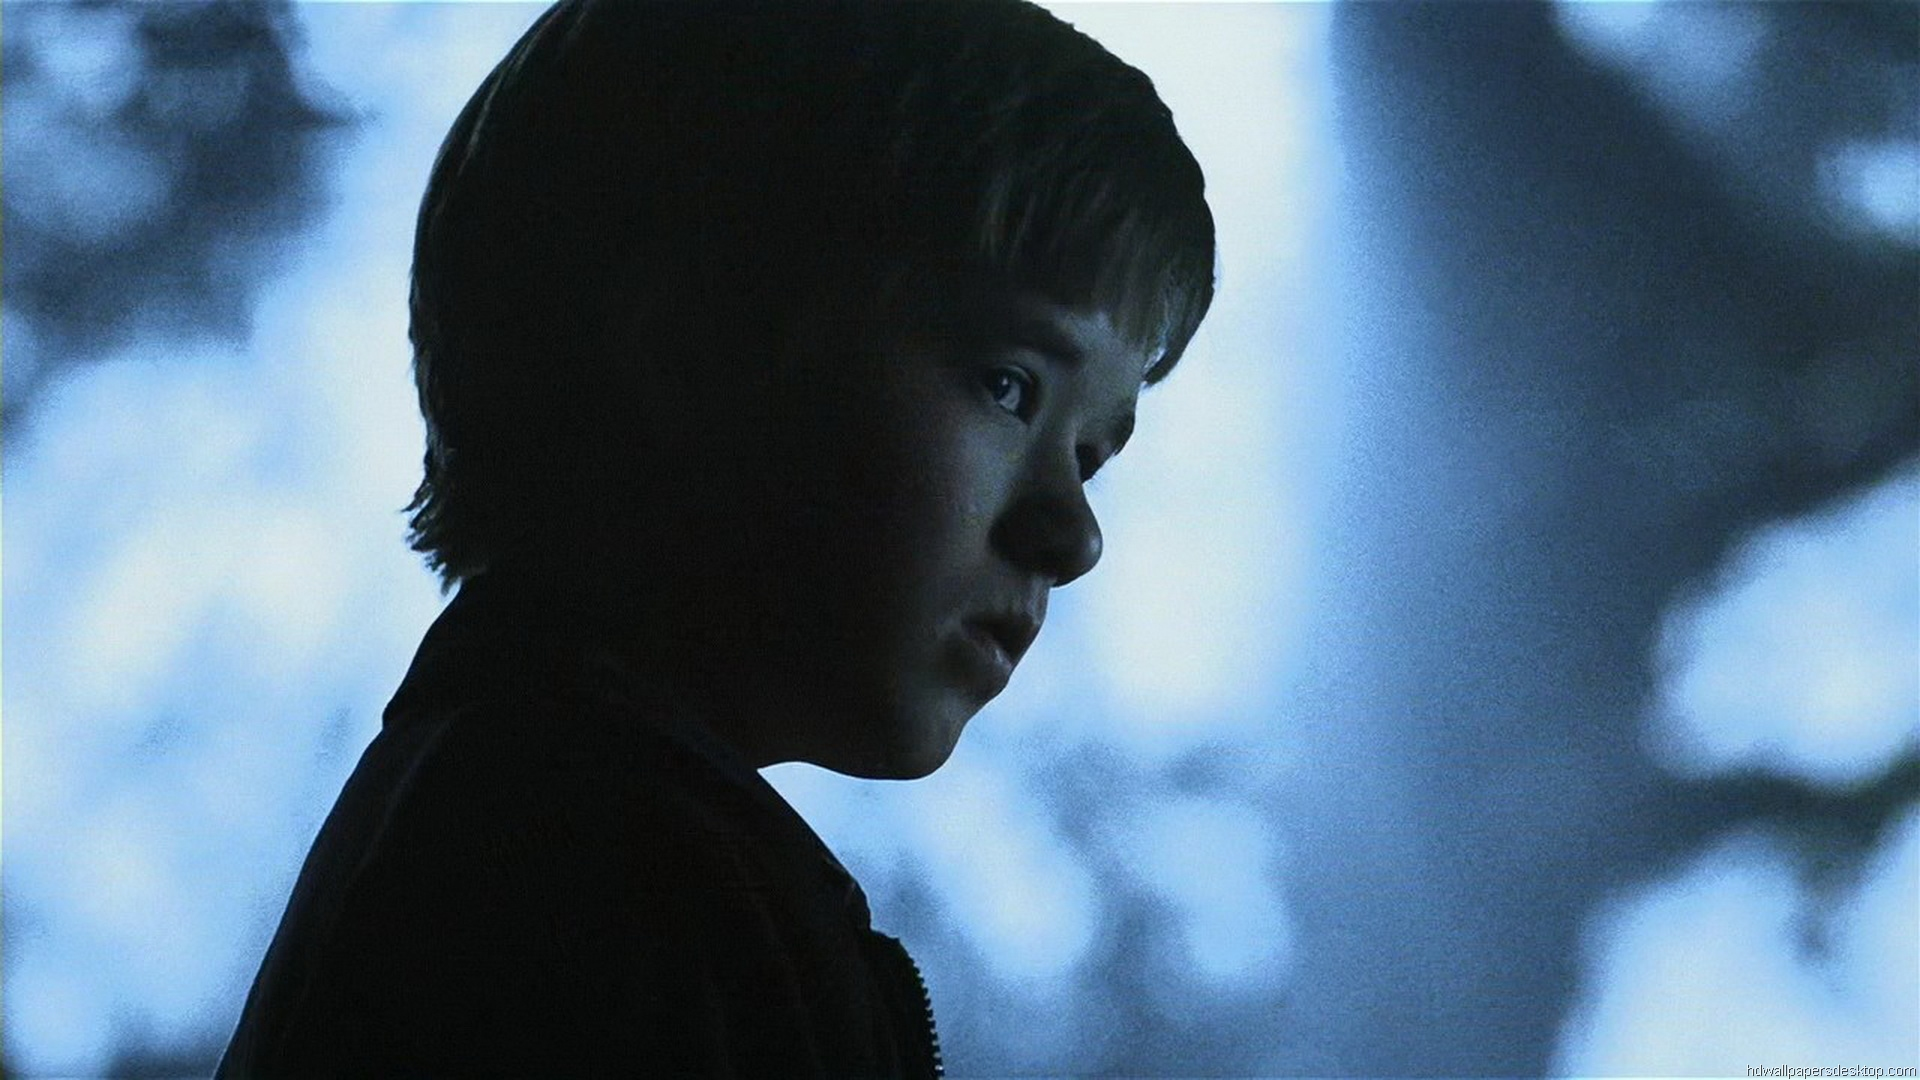
\includegraphics[width=\paperwidth]{images/ai.jpg}
 }
\setbeamercolor{item}{fg=black!70}
\begin{frame}
    \frametitle{Inteligência \hfill\hfill \linebreak Artificial}
\begin{columns}
    \column{\dimexpr 0.6\paperwidth-10pt}
    $\;$
    \column{\dimexpr 0.5\paperwidth-10pt}

    \bfseries \begin{itemize}
        \setlength\itemsep{1em}
        \item \color{black} IA Simbólica
        \item Programação Lógica
        \item Sistema Especialistas
        \item Inteligência Computacional
        \item Aprendizado de Máquinas
    \end{itemize}

\end{columns}
\end{frame}
}

\begin{frame}
    \frametitle{Sistemas Especialistas}
    \begin{itemize}
        \setlength\itemsep{1em}
        \item Anos 70 e 80
        \item Baseados no conhecimento de especialistas do problema.
        \item Aplicação limitada.
        \item Motores de Inferência, Árvores de Decisão, Base de
        Conhecimento, Representação de Conhecimento.
    \end{itemize}
\end{frame}

\begin{frame}
    \frametitle{Raciocínio sobre Incerteza}
    \begin{itemize}
        \setlength\itemsep{1em}
        \item Decidir sobre um problema mesmo com falta de dados,
        ou dados incompletos.
        \item Sistemas Especialistas começam a falhar.
        \item Respostas aproximadas.
        \item Adaptabilidade.
    \end{itemize}
\end{frame}

\begin{frame}
    \frametitle{Lógica Fuzzy}
    \begin{itemize}
        \setlength\itemsep{1em}
        \item A verdade tem um valor entre 0 e 1.
        \item Sistemas são definidos por especialistas.
        \item Diversas aplicações de sucesso.
    \end{itemize}
\end{frame}

\begin{frame}
    \frametitle{Aprendizado}
    \begin{itemize}
        \setlength\itemsep{1em}
        \item Inspirado pelas teorias de Donal Hebb sobre comportamento
        das células.
        \item Sistemas computacionais com aprendizado são programados
        para aprender a solucionar um problema.
        \item Para aprender a solucionar um problema, é necessário que
        o problema seja conhecido pelo sistema.
        \item É possível aprender a partir de uma comparação com uma
        respostas conhecida (supervisão), ou a partir de um resultado
        esperado (sem supervisão).
    \end{itemize}
\end{frame}

\begin{frame}
    \frametitle{Machine Learning}
    \begin{itemize}
        \setlength\itemsep{1em}
        \item Estudo e construção de algoritmos que podem aprender
        e fazer predições baseados nesse aprendizado.
        \item Inclui elementos de computação, estatística, matemática,
        \emph{data mining}, neurociências e outros.
        \item Baseado na ideia de que, assim como humanos, os
        sistemas podem ser aperfeiçoados a partir de experiência.
    \end{itemize}
\end{frame}

\begin{frame}
    \frametitle{Perceptron}

\tikzset{basic/.style={draw,fill=blue!20,text width=1em,text badly centered}}
\tikzset{input/.style={basic,circle}}
\tikzset{weights/.style={basic,rectangle}}
\tikzset{functions/.style={basic,circle,fill=blue!10}}

    \begin{tikzpicture}[overlay, xshift=0.6\paperwidth]
        \node[functions] (center) {};
        \node[below of=center,font=\scriptsize,text width=4em] {Activation function};
        \draw[thick,color=black] (0.5em,0.5em) -- (0,0.5em) -- (0,-0.5em) -- (-0.5em,-0.5em);
        \draw[color=black!50] (0em,0.75em) -- (0em,-0.75em);
        \draw[color=black!50] (0.75em,0em) -- (-0.75em,0em);
        \node[right of=center] (right) {};
            \path[draw,->] (center) -- (right);
        \node[functions,left=3em of center] (left) {\color{black} $\sum$};
            \path[draw,->] (left) -- (center);
        \node[weights,left=3em of left] (2) {\color{black} $w_2$} -- (2) node[input,left of=2] (l2) {\color{black} $x_2$};
            \path[draw,->] (l2) -- (2);
            \path[draw,->] (2) -- (left);
        \node[below of=2] (dots) {$\vdots$} -- (dots) node[left of=dots] (ldots) {$\vdots$};
        \node[weights,below of=dots] (n) {\color{black} $w_n$} -- (n) node[input,left of=n] (ln) {\color{black} $x_n$};
            \path[draw,->] (ln) -- (n);
            \path[draw,->] (n) -- (left);
        \node[weights,above of=2] (1) {\color{black} $w_1$} -- (1) node[input,left of=1] (l1) {\color{black} $x_1$};
            \path[draw,->] (l1) -- (1);
            \path[draw,->] (1) -- (left);
        \node[weights,above of=1] (0) {\color{black} $w_0$} -- (0) node[input,left of=0] (l0) {\color{black} $1$};
            \path[draw,->] (l0) -- (0);
            \path[draw,->] (0) -- (left);
        \node[below of=ln,font=\scriptsize] {inputs};
        \node[below of=n,font=\scriptsize] {weights};
    \end{tikzpicture}
\end{frame}

\begin{frame}
    \frametitle{O Problema do XOR}

    \begin{tikzpicture}[overlay, remember picture, scale=3,
            xshift=1.8cm, yshift=-0.6cm]
        \filldraw[color=black,fill=red]  (0,0) circle (0.2)
            node [color=white] {(0,0)};
        \filldraw[color=black,fill=cyan] (1,0) circle (0.2)
            node [color=white] {(1,0)};
        \filldraw[color=black,fill=red]  (1,1) circle (0.2)
            node [color=white] {(1,1)};
        \filldraw[color=black,fill=cyan] (0,1) circle (0.2)
            node [color=white] {(0,1)};
        \draw[-, color=white, dotted, very thick]
            (-0.2, 1.5) -- (1.6, -0.2)
        ;
    \end{tikzpicture}
\end{frame}

\begin{frame}
    \frametitle{Multi-Layer Perceptron}
\tikzset{%
  every neuron/.style={
    circle,
    draw,
    minimum size=0.7cm
  },
  neuron missing/.style={
    draw=none,
    scale=1,
    text height=0.333cm,
    execute at begin node=\color{white}$\vdots$
  },
}

\begin{tikzpicture}[overlay,xshift=3.8cm, yshift=-1cm, x=1.5cm, y=1.5cm, >=stealth, yscale=0.6]

\foreach \m/\l [count=\y] in {1,2,3,missing,4}
  \node [every neuron/.try, neuron \m/.try] (input-\m) at (0,2.5-\y) {};

\foreach \m [count=\y] in {1,missing,2}
  \node [every neuron/.try, neuron \m/.try ] (hidden-\m) at (2,2-\y*1.25) {};

\foreach \m [count=\y] in {1,missing,2}
  \node [every neuron/.try, neuron \m/.try ] (output-\m) at (4,1.5-\y) {};

\foreach \l [count=\i] in {1,2,3,n}
  \draw [<-] (input-\i) -- ++(-1,0)
    node [above, midway] {$I_\l$};

\foreach \l [count=\i] in {1,n}
  \node [above] at (hidden-\i.north) {$H_\l$};

\foreach \l [count=\i] in {1,n}
  \draw [->] (output-\i) -- ++(1,0)
    node [above, midway] {$O_\l$};

\foreach \i in {1,...,4}
  \foreach \j in {1,...,2}
    \draw [->] (input-\i) -- (hidden-\j);

\foreach \i in {1,...,2}
  \foreach \j in {1,...,2}
    \draw [->] (hidden-\i) -- (output-\j);

\foreach \l [count=\x from 0] in {Input, Hidden, Ouput}
  \node [align=center, above] at (\x*2,2) {\l \\ layer};

\end{tikzpicture}
\end{frame}

\begin{frame}
    \frametitle{Solução do XOR}
    \begin{center}
        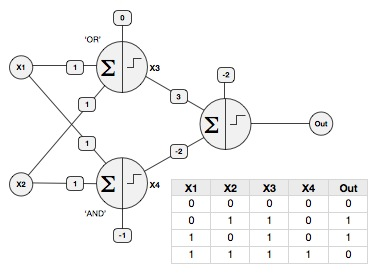
\includegraphics[height=.6\paperheight]{images/xor_mlp.jpg}
    \end{center}
\end{frame}

\begin{frame}
    \frametitle{Modelos de Aprendizagem}
    \begin{itemize}
        \setlength\itemsep{1em}
        \item Aprendizado supervisionado: utiliza um \textbf{tutor},
        que mostra qual o resultado esperado para um conjunto de
        valores de entrada.
        \item Aprendizado não supervisionado: avalia o resultado obtido
        para uma determinada entrada, sem um \textbf{tutor}.
    \end{itemize}
\end{frame}

\begin{frame}
    \frametitle{Outros Métodos de Machine Learning}
    \begin{itemize}
        \setlength\itemsep{1em}
        \item Self Organizing Maps
        \item Principal Component Analisys
        \item Support Vector Machines
        \item Modelos Ocultos de Markov
        \item Modelos de Bayes
        \item Convolutional Neural Networks
    \end{itemize}
\end{frame}

\begin{frame}
    \frametitle{Deep Learning}
    \vfill
    Envolve diversos algoritmos adaptativos de extração de características
    e reconhecimento de padrões.
    \vfill
    Necessita de uma grande quantidade de dados, e um enorme poder de
    processamento.
    \vfill
\end{frame}

\begin{frame}
    \frametitle{O que possibilitou o Deep Learning?}
    \vfill
    \begin{itemize}
        \setlength\itemsep{1em}
        \item{\emph{Hardware} muito mais potente, GPUs.}
        \item{Novos algoritmos de treinamento, como as MLP e as redes convolutivas.}
    \end{itemize}
    \vfill
    Exatamente como previsto por Minski e Pappert...
\end{frame}

\begin{frame}
    \frametitle{Implementando Machine Learning}
    \begin{itemize}
        \setlength\itemsep{1em}
        \item Theano (Python)
        \item Torch (Lua)
        \item TensorFlow (Python - Google)
        \item Caffe (Pyhton)
    \end{itemize}
\end{frame}

\begin{frame}
    \frametitle{Problemas em Aberto}
    \begin{itemize}
        \setlength\itemsep{1em}
        \item{Como organizar e formatar os dados?}
        \item{Que dados são relevantes ao problema?}
        \item{O que a rede neural aprendeu?}
    \end{itemize}
\end{frame}

\begin{frame}[b]
    \begin{center}
    \Huge \bfseries Muito Obrigado!
    \end{center}
    \vfill
    \hfill \textbf{rafasgj@gmail.com} \\
    \hfill \footnotesize{http://rafaeljeffman.com?lectures}
\end{frame}

\end{document}
